\documentclass[preview]{standalone}
\usepackage{tikz}
\usepackage{tikz-qtree}
\usepackage{subcaption}
\usetikzlibrary{arrows,automata, positioning, patterns}

\begin{document}
\begin{figure}
  \begin{subfigure}{.3\linewidth}
     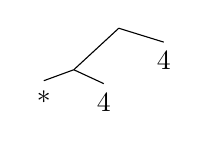
\begin{tikzpicture} 
       \tikzset{level distance=15pt, sibling distance=10pt}
       \Tree [[  * 4 ] 4 ]
     \end{tikzpicture}
  \end{subfigure}
  \begin{subfigure}{.3\linewidth}
     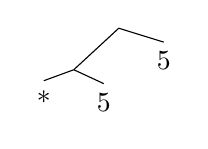
\begin{tikzpicture} 
       \tikzset{level distance=15pt, sibling distance=10pt}
       \Tree [[  * 5 ] 5 ]
     \end{tikzpicture}
  \end{subfigure}
  \begin{subfigure}{.3\linewidth}
     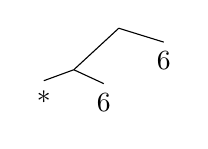
\begin{tikzpicture} 
       \tikzset{level distance=15pt, sibling distance=10pt}
       \Tree [[  * 6 ] 6 ]
     \end{tikzpicture}
  \end{subfigure}

  \begin{subfigure}{.3\linewidth}
     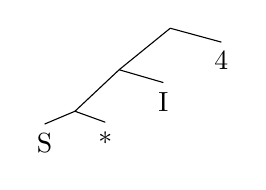
\begin{tikzpicture} 
       \tikzset{level distance=15pt, sibling distance=10pt}
       \Tree [[[  S * ] I ] 4 ] 
     \end{tikzpicture}
  \end{subfigure}
   \begin{subfigure}{.3\linewidth}
     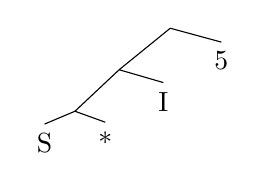
\begin{tikzpicture} 
       \tikzset{level distance=15pt, sibling distance=10pt}
       \Tree [[[  S * ] I ] 5 ] 
     \end{tikzpicture}
  \end{subfigure}
  \begin{subfigure}{.3\linewidth}
     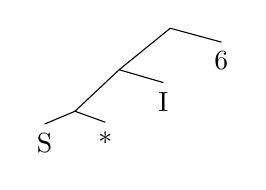
\begin{tikzpicture} 
       \tikzset{level distance=15pt, sibling distance=10pt}
       \Tree [[[  S * ] I ] 6 ] 
     \end{tikzpicture}
  \end{subfigure}
\end{figure}
 
\end{document}


